\chapter{Aplicación a SPY}
\label{cap:spy}

% Fuente única de cifras: notebooks/STRATA_marco_practico.ipynb (panel canónico de 10) y sus JSON en
% outputs/experiments/. Toda cifra trazada a su JSON en el caption de su tabla.

El agente solo (M5) acierta sobre SPY el $0{,}366$ de las direcciones y pierde dinero: ese es el punto de partida. SPY es el ETF que replica el S\&P~500, el índice de las quinientas mayores empresas cotizadas de Estados Unidos. Tiene un \emph{leverage effect} de índice amplio y por eso el régimen adquiere contenido direccional (Sección~\ref{sec:strata-ram}) según lo que dice la literatura lo que lo hace un buen candidato para mostrar la aplicabilidad de nuestro sistema. Sobre él construimos la cadena entera: la intervención y su anatomía, las seis estrategias que compiten y la atribución de lo que STRATA rescata.



\section{La intervención en detalle}
\label{sec:spy-anatomia}

Fijamos primero el protocolo. Con \texttt{signal\_lag}${}=1$ (capítulo~\ref{cap:strata}), la posición del día $t$ se enfrenta al retorno del día $t+1$, nunca al del propio día. Calibramos los detectores una sola vez sobre 2000-01-01 a 2024-09-30 y cerramos sus umbrales antes de ver la evaluación, que arranca el 2024-10-01, ya pasado el corte de conocimiento del modelo de lenguaje: así el agente no pudo memorizar esas decisiones.

Conviven dos ventanas que nunca mezclamos. El OOS completo ($n = 401$) sirve a las estrategias que no entrenan: el agente, la regla y las dos triviales. La ventana desplegable ($n = 251$) es la que queda tras un arranque de ciento cincuenta días de \emph{walk-forward} de origen rodante, y la usan las estrategias que reentrenan a diario, con embargo${}=1$ por su horizonte de etiqueta de un día (Tashman 2000 \cite{tashman2000}; López de Prado 2018 \cite{lopezdeprado2018}).

Los tres detectores descansan en modelos clásicos calibrados en esa ventana. El régimen lo da un HMM gaussiano de tres estados ($K = 3$), que etiquetamos Calma, Estrés y Crisis (Rabiner 1989 \cite{rabiner1989}); $K$ no se elige a posteriori, lo fija una selección de modelo ex ante. La volatilidad la sigue un GARCH(1,1) de innovaciones $t$ de Student, cuya cola pesada recoge los movimientos extremos que una normal subestima (Bollerslev 1987 \cite{bollerslev1987}). El cambio estructural lo vigila un BOCPD en línea, que actualiza con cada dato la probabilidad de cuántos días lleva el agente sin cambiar de conducta, sin mirar el futuro (Adams y MacKay 2007 \cite{adams2007}). Sus umbrales de disparo son cuantiles de la calibración. Con esto fijado, entramos en la mecánica de la intervención sobre SPY.

El \emph{leverage} de un activo lo medimos con la correlación de Black, $\mathrm{lev} = \operatorname{corr}(r_t,\ \mathrm{RV}^{21}_{t+1} - \mathrm{RV}^{21}_t)$, entre el retorno de hoy y el cambio de la volatilidad realizada a veintiún días: es negativa cuando una caída eleva la volatilidad del día siguiente. La Figura~\ref{fig:mp-regimenes-spy} muestra los tres regímenes pintados sobre el precio de SPY. Esto es escriptivo, empleamos el camino de máxima verosimilitud de Viterbi (Anexo~\ref{anx:viterbi}), una decodificación retrospectiva sobre toda la serie; el detector RAM no lo usa para evitar look ahead en tiempo real lee la probabilidad filtrada causal del estado.Una precisión gobierna toda la lectura: en la calibración el retorno del mismo día baja con el régimen, pero la fracción de días al alza del día siguiente ronda $0{,}5$ incluso en Crisis. El régimen separa por volatilidad y coincide con la caída del mismo día, no anticipa el signo de mañana.

\begin{figure}[htbp]
\centering
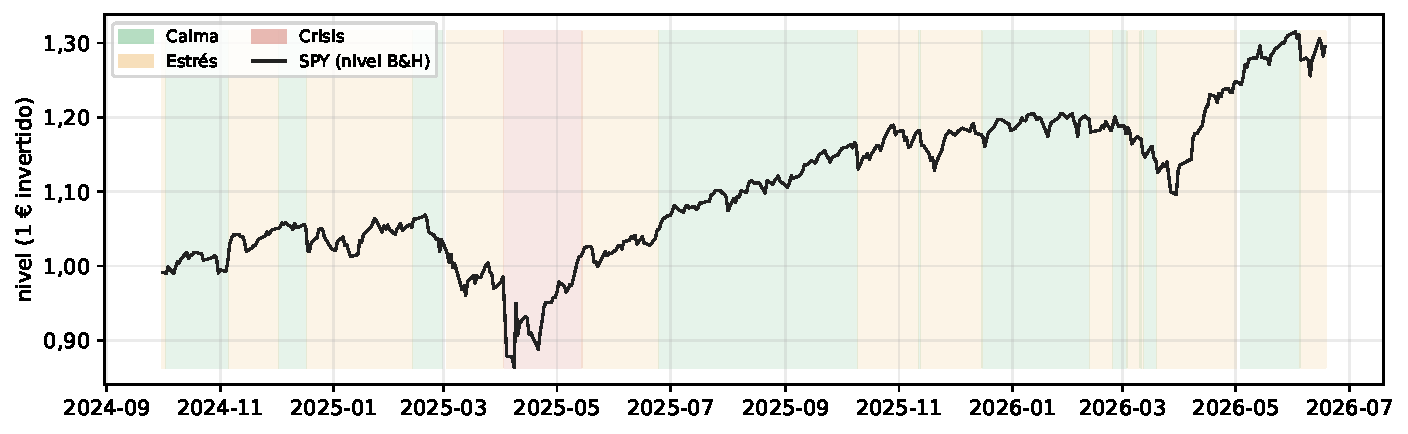
\includegraphics[width=0.74\textwidth]{figuras/cap4_regimenes_spy}
\caption{Regímenes del HMM ($K = 3$) sobre el precio de SPY en el periodo de evaluación. Calma (volatilidad baja, retorno medio positivo), Estrés (intermedio) y Crisis (volatilidad alta, retorno medio negativo) ordenan por la firma del \emph{leverage effect}. El sombreado marca el régimen vigente cada día; la coincidencia régimen$\leftrightarrow$caída es contemporánea, no predictiva.}
\label{fig:mp-regimenes-spy}
\end{figure}

Los tres detectores miran ejes ortogonales de la decisión del agente. RAM lee el régimen y comprueba si la dirección de la apuesta concuerda con el estado vigente: su \emph{score} es la probabilidad que el HMM pone en que el agente apuesta contra el régimen, y dispara cuando $\mathrm{RAM}_t \ge \tau = 0{,}50$. PSA vigila con BOCPD si el agente cambia de criterio de forma estructural (Adams y MacKay 2007 \cite{adams2007}). GSO contrasta el tamaño de la posición con la volatilidad del GARCH (Bollerslev 1986 \cite{bollerslev1986}). Cuando RAM dispara, la intervención reorienta la posición al signo del régimen, fijado por un prior calibrado por activo a partir de la media del retorno de cada estado, nunca por una regla del tipo ``Crisis implica corto'' escrita a mano.

Sobre SPY actúa una sola supervisión (Tabla~\ref{tab:mp-detectores}). RAM dispara casi un tercio de los días y acierta más al intervenir que el agente al que corrige; PSA dispara dos días y GSO ninguno. El motivo es que el agente mantiene una posición casi constante sobre SPY, corta la mayor parte de los días, de modo que sus \emph{scores} de cambio y de tamaño quedan por debajo de los umbrales de calibración. PSA y GSO son detectores inertes como reglas sobre este activo, un hallazgo que registramos. La atribución de P\&L cierra la lectura: todo el rescate acumulado sale de los días en que RAM dispara, y PSA y GSO aportan exactamente cero.

\begin{table}[htbp]
\centering
\caption{Actividad de los tres detectores sobre el OOS completo de SPY ($n = 401$ días). ``Acierto'' es la fracción de direcciones correctas en los días en que el detector dispara; el P\&L de rescate es el acumulado de la intervención en esos días. PSA y GSO apenas disparan: su columna de acierto no aplica. Fuente: \texttt{spy\_intervention\_anatomy.json}.}
\label{tab:mp-detectores}
\begin{tabular}{lrrrr}
\toprule
Detector & Tasa de disparo & Acierto M8 & Acierto M5 & P\&L de rescate \\
\midrule
\textbf{RAM} (régimen) & $\mathbf{30{,}2\%}$ & $\mathbf{0{,}587}$ & $0{,}413$ & $\mathbf{+0{,}312}$ \\
PSA (cambio estructural) & $0{,}5\%$ & --- & --- & $0{,}000$ \\
GSO (volatilidad) & $0{,}0\%$ & --- & --- & $0{,}000$ \\
\bottomrule
\end{tabular}
\end{table}

Que RAM acierte al intervenir no es casualidad, y la Figura~\ref{fig:mp-scores-detectores} lo deja ver. En los días en que RAM está alto, seguir el régimen bate a seguir al agente; cuando RAM está bajo, la ventaja se diluye y la intervención no se activa. El detector funciona como una compuerta: deja pasar la decisión del agente salvo cuando choca con el régimen, y solo entonces la corrige. En SPY esa compuerta es todo el mecanismo de la regla, porque el canal de régimen es el único que se enciende.

\begin{figure}[htbp]
\centering
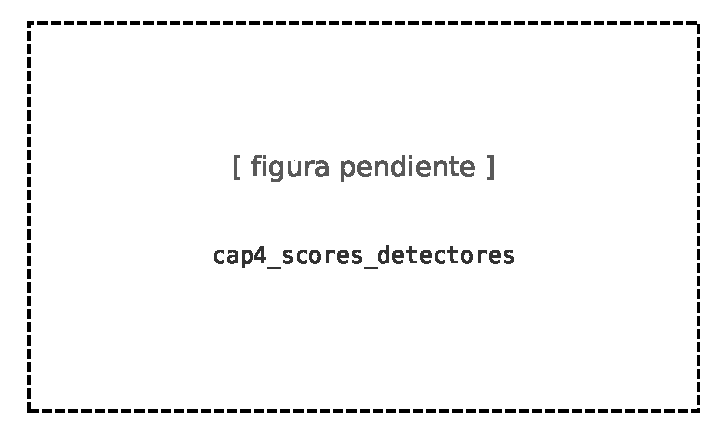
\includegraphics[width=0.74\textwidth]{figuras/cap4_scores_detectores}
\caption{Distribución de los \emph{scores} de RAM, PSA y GSO sobre el OOS de SPY, con su umbral de disparo marcado (RAM $\tau = 0{,}50$, PSA $P_{95} = 0{,}023$, GSO $P_{95} = 2{,}371$). El \emph{score} de RAM es bimodal y cruza el umbral con frecuencia; los de PSA y GSO se acumulan muy por debajo del suyo, de ahí que apenas disparen.}
\label{fig:mp-scores-detectores}
\end{figure}

La intervención puede ejecutarse de tres maneras. Puede abstenerse los días dudosos cerrando la posición, reducir el tamaño a la mitad, o reorientar la dirección al signo del régimen, el modo que llamamos \emph{override}. La Tabla~\ref{tab:mp-variantes} compara los tres sobre los días en mercado ($n = 232$). El \emph{override}, que adoptamos como modo canónico, gana en acierto y en Sharpe; abstenerse y reducir apenas se distinguen del agente sin tocar. El valor está en corregir activamente la dirección cuando choca con el régimen, no en limitarse a evitar el riesgo.

\begin{table}[htbp]
\centering
\caption{Modos de intervención de M8 sobre SPY (días en mercado, $n = 232$). El modo canónico (\emph{override}) reorienta la posición al signo del régimen; las alternativas se abstienen o reducen el tamaño. En negrita, el modo adoptado. Fuente: \texttt{spy\_intervention\_variants.json}.}
\label{tab:mp-variantes}
\begin{tabular}{lrrr}
\toprule
Modo & Accuracy & Sharpe & Capital \\
\midrule
\textbf{Override} (canónico) & $\mathbf{0{,}478}$ & $\mathbf{-0{,}46}$ & $\mathbf{0{,}94\times}$ \\
Abstención & $0{,}401$ & $-2{,}10$ & $0{,}81\times$ \\
Reducir a la mitad & $0{,}397$ & $-2{,}75$ & $0{,}75\times$ \\
M5 (agente sin tocar) & $0{,}397$ & $-3{,}07$ & $0{,}70\times$ \\
\bottomrule
\end{tabular}
\end{table}

La anatomía de esas intervenciones está en la matriz de confusión de la Figura~\ref{fig:mp-confusion-spy}: unas corrigen al agente cuando apostaba contra el régimen, otras meten ruido cuando el agente tenía razón. El saldo neto es positivo porque la intervención no es indiscriminada: crece con la discrepancia entre la apuesta del agente y el signo del régimen. Cuanto más se aleja el agente del estado del mercado, con más fuerza actúa la regla, y son justo esos días de discrepancia grande los que aportan el grueso del rescate.

\begin{figure}[htbp]
\centering
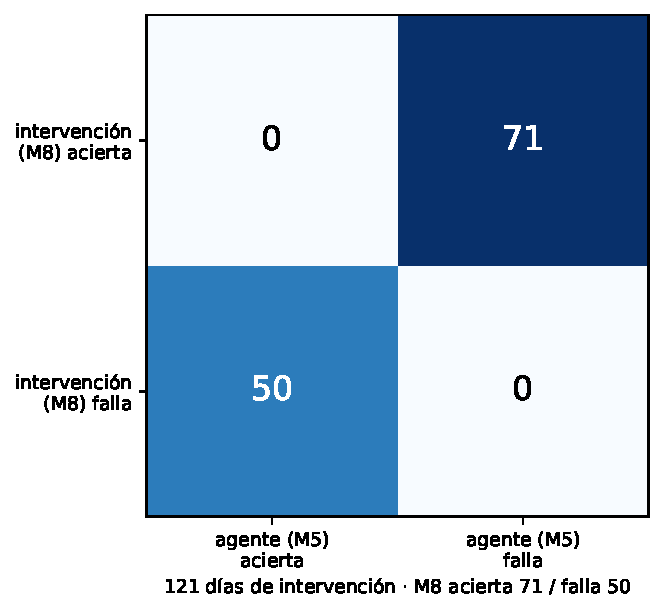
\includegraphics[width=0.7\textwidth]{figuras/cap4_confusion_spy}
\caption{Matriz de confusión de la intervención sobre SPY: dirección del agente (M5) frente a dirección tras intervenir (M8), sobre las $121$ intervenciones. La diagonal de rescate ($71$ aciertos de la intervención cuando el agente fallaba) supera a la de daño ($50$).}
\label{fig:mp-confusion-spy}
\end{figure}

\section{Comparación de las seis estrategias}
\label{sec:spy-estrategias}

Sobre el agente comparamos las seis estrategias ya introducidas en el capítulo anterior. M5 es el agente sin supervisar. M8 es la regla determinista de la intervención. M10 es el meta-learner, un ensemble de diez XGBoost sobre las veintidós características del agente y de STRATA. AutoML deja que H2O busque por reentreno entre GBM, XGBoost y su apilamiento. Las dos referencias triviales son comprar y mantener (B\&H) y la clase mayoritaria del pasado (ZeroR): marcan el listón que cualquier pretensión de habilidad debe superar. La Tabla~\ref{tab:mp-spy} las reúne sobre la ventana desplegable.

\begin{table}[htbp]
\centering
\caption{Las seis estrategias sobre SPY, ventana desplegable ($n = 251$, \texttt{signal\_lag}${}=1$). Accuracy direccional, Sharpe anualizado, máxima caída, ratio de Calmar (Young 1991 \cite{young1991}) y capital final por euro invertido. En negrita, la mejor en cada columna. Fuente: \texttt{automl\_runs/panel\_mm25\_inclGBM-XGB-SE\_AUC\_emb1\_N0-150\_step21\_kfold\_seed42.json}.}
\label{tab:mp-spy}
\begin{tabular}{lrrrrr}
\toprule
Estrategia & Accuracy & Sharpe & Máx.\ caída & Calmar & Capital \\
\midrule
\textbf{AutoML} (búsqueda H2O) & $\mathbf{0{,}574}$ & $\mathbf{+2{,}68}$ & $\mathbf{-5{,}5\%}$ & $\mathbf{6{,}93}$ & $\mathbf{1{,}38\times}$ \\
ZeroR (clase mayoritaria) & $0{,}566$ & $+2{,}21$ & $-9{,}8\%$ & $3{,}10$ & $1{,}30\times$ \\
B\&H (comprar y mantener) & $0{,}566$ & $+2{,}21$ & $-9{,}8\%$ & $3{,}10$ & $1{,}30\times$ \\
M10 (meta-learner XGBoost) & $0{,}494$ & $-0{,}60$ & $-16{,}1\%$ & $-0{,}50$ & $0{,}92\times$ \\
M8 (regla STRATA) & $0{,}442$ & $-0{,}46$ & $-15{,}2\%$ & $-0{,}39$ & $0{,}94\times$ \\
M5 (agente solo) & $0{,}366$ & $-3{,}07$ & $-30{,}2\%$ & $-1{,}00$ & $0{,}70\times$ \\
\bottomrule
\end{tabular}
\end{table}

Leída de abajo arriba, podemos decir cada capa rescata a la anterior. La regla recupera al agente y le recorta a la mitad la máxima caída; el meta-learner sube otro escalón en accuracy; AutoML llega arriba y gana en todas las columnas, también a las dos triviales. El rescate es significativo en los tres casos, contrastado con el McNemar pareado sobre los aciertos diarios frente al agente (McNemar 1947 \cite{mcnemar1947}). Los tres rescatan al agente, y el rescate aguanta el test.

La victoria sobre la trivial necesita un matiz. El mismo McNemar de AutoML frente a ZeroR no separa a las dos: no hay potencia en una ventana de doscientos cincuenta días. La ventaja de AutoML sobre el mercado pasivo es real en punto pero nominal en significancia, y tiene una explicación económica: SPY es mayormente beta de mercado, el periodo de evaluación fue alcista, e ir largo capturó esa subida. La Figura~\ref{fig:mp-equity-spy} hace visible la diferencia, y el Sharpe deflactado (López de Prado 2018 \cite{lopezdeprado2018}; Bailey y López de Prado 2014 \cite{bailey2014}) la pone en contexto. El DSR confirma esa lectura: solo el de AutoML se acerca a uno, mientras los de M10 y el agente quedan pegados a cero. AutoML es el único de los modelos cuyo Sharpe sobrevive al ajuste por número de pruebas.

\begin{figure}[htbp]
\centering
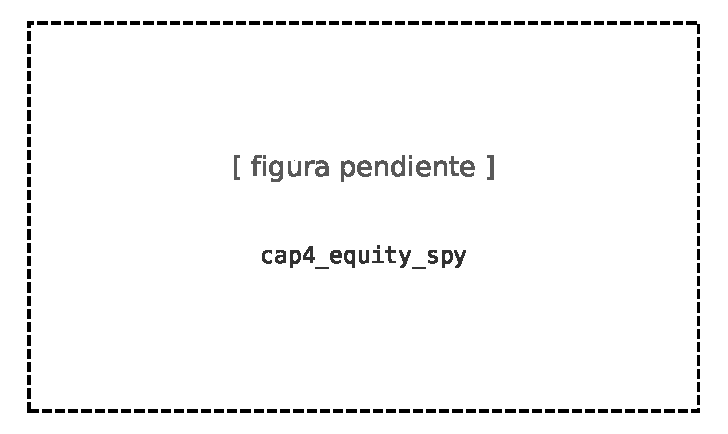
\includegraphics[width=0.74\textwidth]{figuras/cap4_equity_spy}
\caption{Curvas de capital de las seis estrategias sobre SPY (ventana desplegable, $n = 251$ días, un euro inicial). AutoML (línea destacada) supera a las dos referencias triviales en Sharpe ($+2{,}68$ frente a $+2{,}21$), en máxima caída ($-5{,}5\%$ frente a $-9{,}8\%$) y en capital final ($1{,}38\times$ frente a $1{,}30\times$); el agente solo (M5) termina en $0{,}70\times$. La ventaja sobre la trivial es nominal (McNemar AutoML vs ZeroR $p = 0{,}90$).}
\label{fig:mp-equity-spy}
\end{figure}

Sobre un único activo, el intervalo de confianza del $\Delta$Sharpe de la regla frente al agente cruza el cero. El resultado en riesgo que no alcanza significancia a este nivel, lo comprobamos en una muestra mayor de activos en el siguiente capítulo.

\section{El rescate sobre SPY}
\label{sec:spy-rescate}

Ya vimos que sobre SPY el régimen (Sección~\ref{sec:spy-anatomia}) es el único que rescata. La preguna que nos queda por responder es: ¿usa de verdad el aprendiz las señales de STRATA, o gana por otro lado? La ablación lo responde. Al quitar PSA y GSO de las características, la accuracy de AutoML baja (Tabla~\ref{tab:mp-ablacion}): aunque PSA y GSO casi no disparen como reglas, sus \emph{scores} continuos informan al modelo. Las características de Shapley (Lundberg y Lee 2017 \cite{lundberg2017}) lo confirman, y aquí etiquetamos cada cuota con su modelo y su ventana porque no son el mismo objeto. Sobre el ensemble M10 ($n = 251$), la cuota de las features de STRATA es $0{,}71$. Sobre el \emph{leader} de AutoML ($n = 401$, otro modelo y otra ventana), es $0{,}565$ por árbol y $0{,}564$ por permutación. Las dos cuotas superan la mitad y colocan los detectores por delante de las características del propio agente.

Ya vimos que sobre SPY el régimen (Sección~\ref{sec:spy-anatomia}) es el único que rescata. La pregunta que nos queda por responder es: ¿usa de verdad el aprendiz las señales de STRATA, o gana por otro lado? La ablación lo responde. Quitamos PSA y GSO de las características y reentrenamos: la accuracy de AutoML baja (Tabla~\ref{tab:mp-ablacion}). Aunque esos dos detectores casi nunca disparen como reglas, sus \emph{scores} continuos llevan información que el modelo aprovecha porque sin ellos rinde peor.

Los valores de Shapley (Lundberg y Lee 2017 \cite{lundberg2017}) lo confirman desde otro ángulo: reparten la importancia total del modelo entre las quince características del agente y las siete de STRATA. Aunque STRATA aporta solo siete de las veintidós, se lleva más de la mitad del peso. Damos la cuota etiquetada con su modelo y su ventana, porque no son el mismo objeto: sobre el ensemble M10 (ventana desplegable, $n = 251$) vale $0{,}71$; sobre el \emph{leader} de AutoML ($n = 401$, otro modelo) vale $0{,}565$ por árbol y $0{,}564$ por permutación, dos cálculos distintos que coinciden. En todos los casos supera la mitad: el aprendiz coloca los detectores por delante de las características del propio agente. Las dos pruebas apuntan a lo mismo, ablación y atribución: el aprendiz sí se apoya en STRATA.


\begin{table}[htbp]
\centering
\caption{Ablación de detectores sobre SPY (ventana desplegable, $n = 251$). El conjunto canónico usa las veintidós características; ``sin PSA+GSO'' deja solo el canal de régimen entre los detectores. AutoML degrada al quitar PSA+GSO, prueba de que usa sus \emph{scores}. Fuente: \texttt{automl\_ablation\_detectors.json}, \texttt{detector\_ablation\_panel.json}.}
\label{tab:mp-ablacion}
\begin{tabular}{lrr}
\toprule
Conjunto de características & Accuracy AutoML & Accuracy M10 \\
\midrule
\textbf{ALL22} (canónico) & $\mathbf{0{,}574}$ & $0{,}494$ \\
sin PSA+GSO & $0{,}550$ & $0{,}514$ \\
\bottomrule
\end{tabular}
\end{table}


La objeción más natural es que los umbrales se eligieran para que el resultado saliera bien. El barrido completo lo descarta (Figura~\ref{fig:mp-sensibilidad}): la accuracy apenas se mueve alrededor del valor canónico, ni al variar el umbral $\tau$ de RAM en M8 ni el umbral de decisión del meta-learner. El resultado no cuelga de un punto afortunado, sino que descansa sobre una meseta estable; es lo contrario de un ajuste fino al periodo de evaluación y es lo que nos protege de la sospecha de sobreajuste.


\begin{figure}[htbp]
\centering
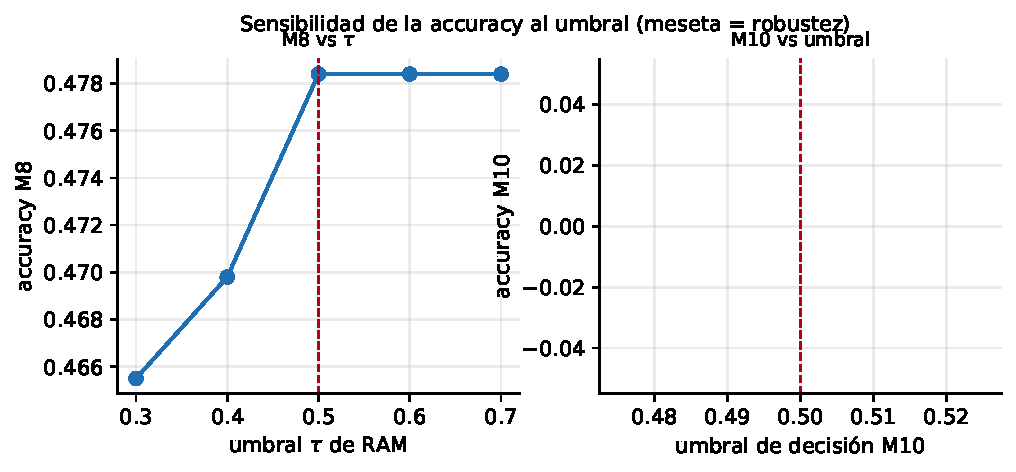
\includegraphics[width=0.74\textwidth]{figuras/cap4_sensibilidad_umbrales}
\caption{Sensibilidad de la accuracy al umbral de decisión sobre SPY: M8 frente a $\tau$ del detector RAM y M10 frente a su umbral de probabilidad. Las dos curvas son planas en una meseta alrededor del valor canónico (marcado), señal de robustez y no de ajuste a un punto.}
\label{fig:mp-sensibilidad}
\end{figure}

Para concluir, sobre SPY el mecanismo es transparente y el agente, sin supervisión, pierde con holgura. La intervención por régimen lo corrige de forma significativa, la derivada aprendida supera a la trivial en este punto apoyándose en las señales de STRATA, y todo descansa sobre una meseta robusta de umbrales. A nivel de un único activo, sin embargo, la corrección de riesgo no alcanza significancia y la victoria sobre la trivial es nominal. Queda la pregunta que enfoca el resto del trabajo: ¿se sostiene el rescate fuera de SPY? El panel de diez activos es el siguiente paso.
